% IMPORTANT

% 
% Install tex distribution
% https://www.latex-project.org/get/
% With Windows, install MikTeX
% 

% Go to Tools/Global Options/Sweave
% Select Weave Rnw files using: knitr
% Select Typeset LaTeX into PDF using: pdfLaTeX







% Load graphicx package in your document's preamble
% Gandrud (2016), p.192

% turn page 90 degrees with lscape Gandrud (2016), p.185

% Create clickable hyperlinks with hyperref package, Gandrud (2016), p. 218

% Use natbib package for bibliography formatting, authoryear for Harvard style , Gandrud (2016), p. 227
% commands to change what information is included in the parentheses, Gandrud (2016), p. 228, table 11.2

% Using saveRDS and readRDS, following 
% https://csgillespie.github.io/efficientR/efficient-inputoutput.html#efficient-data-export-.rdata-or-.rds

% working with knitR and LaTeX
% https://kbroman.org/knitr_knutshell/pages/latex.html
% Command line
% R -e 'library(knitr);knit("knitr_example.Rnw")'

% Create list of packages used, Gandrud (2016), p 218/219

\documentclass[12pt, a4paper]{article}\usepackage[]{graphicx}\usepackage[]{color}
% maxwidth is the original width if it is less than linewidth
% otherwise use linewidth (to make sure the graphics do not exceed the margin)
\makeatletter
\def\maxwidth{ %
  \ifdim\Gin@nat@width>\linewidth
    \linewidth
  \else
    \Gin@nat@width
  \fi
}
\makeatother

\definecolor{fgcolor}{rgb}{0.345, 0.345, 0.345}
\newcommand{\hlnum}[1]{\textcolor[rgb]{0.686,0.059,0.569}{#1}}%
\newcommand{\hlstr}[1]{\textcolor[rgb]{0.192,0.494,0.8}{#1}}%
\newcommand{\hlcom}[1]{\textcolor[rgb]{0.678,0.584,0.686}{\textit{#1}}}%
\newcommand{\hlopt}[1]{\textcolor[rgb]{0,0,0}{#1}}%
\newcommand{\hlstd}[1]{\textcolor[rgb]{0.345,0.345,0.345}{#1}}%
\newcommand{\hlkwa}[1]{\textcolor[rgb]{0.161,0.373,0.58}{\textbf{#1}}}%
\newcommand{\hlkwb}[1]{\textcolor[rgb]{0.69,0.353,0.396}{#1}}%
\newcommand{\hlkwc}[1]{\textcolor[rgb]{0.333,0.667,0.333}{#1}}%
\newcommand{\hlkwd}[1]{\textcolor[rgb]{0.737,0.353,0.396}{\textbf{#1}}}%
\let\hlipl\hlkwb

\usepackage{framed}
\makeatletter
\newenvironment{kframe}{%
 \def\at@end@of@kframe{}%
 \ifinner\ifhmode%
  \def\at@end@of@kframe{\end{minipage}}%
  \begin{minipage}{\columnwidth}%
 \fi\fi%
 \def\FrameCommand##1{\hskip\@totalleftmargin \hskip-\fboxsep
 \colorbox{shadecolor}{##1}\hskip-\fboxsep
     % There is no \\@totalrightmargin, so:
     \hskip-\linewidth \hskip-\@totalleftmargin \hskip\columnwidth}%
 \MakeFramed {\advance\hsize-\width
   \@totalleftmargin\z@ \linewidth\hsize
   \@setminipage}}%
 {\par\unskip\endMakeFramed%
 \at@end@of@kframe}
\makeatother

\definecolor{shadecolor}{rgb}{.97, .97, .97}
\definecolor{messagecolor}{rgb}{0, 0, 0}
\definecolor{warningcolor}{rgb}{1, 0, 1}
\definecolor{errorcolor}{rgb}{1, 0, 0}
\newenvironment{knitrout}{}{} % an empty environment to be redefined in TeX

\usepackage{alltt}
\usepackage{lscape}
\usepackage{graphicx}
\usepackage[utf8]{inputenc}
\usepackage[backend=biber, bibstyle=apa, citestyle=authoryear]{biblatex}
\usepackage{floatrow}
\usepackage[hidelinks]{hyperref}
% \usepackage[authoryear]{natbib}
% \bibliographystyle{apalike}
\usepackage{mathtools}
\usepackage[onehalfspacing]{setspace}
\usepackage[left = 72 pt, right = 72 pt]{geometry}

% \addbibresource{Main.bib}





\title{Effects of CHILDREN's programs}
\author{Laura Huber, Laura Jepsen, Jonathan Kirschner, Rafael Schütz, Yannick Zurl}
\date{27th February 2020}
\IfFileExists{upquote.sty}{\usepackage{upquote}}{}
\begin{document}

\begin{titlepage}
\maketitle
\end{titlepage}

\tableofcontents
\listoftables
\listoffigures

% To have an unnumbered section, place an sterisk in it like this \*{Unnumbered Section}

\section{Introduction}

\section{Outline}
Descriptive statistics\\
- dynamics of selected outcomes\\
- dynamics of real subsidy per institution\\
- dynamics of real total subsidy\\
(- dynamics of real subsidy per individual)\\
(- which variables have largest variance; also relevant for variable selection)\\

Regressions\\

Questions:\\
- effect of healthy meals (DGE criterion) on healthy characteristics\\
- effect of real meals subsidy on number of meals\\
- effect of real trips subsidy on number of trips\\
- effect of real meals subsidy on self-worth and day-to-day skills\\

Methods:\\
- simple, metric\\
- standardized, metric\\
- cumulative logit\\
- with control variables\\
(- without outliers)\\
(- imputed data)\\

Diff in Diff\\

Outlook for CHILDREN/variable selection\\
- double selection \\
- partition analysis\\
(- correlation matrix)\\
(- factor analysis)\\
- general tips\\

Examples\\

Equation\\

\begin{equation}
\label{ModelProdu}
\ln y_{it} = \beta_0 + \beta_k \ln k_{it-1} + \beta_n \ln n_{it} + \beta_m \ln m_{it} + \beta_t D_t + \beta_i D_i + \epsilon_{it}
\end{equation}

List\\

\begin{itemize}
  \item{The firm is not incorporated in the U.S. (FIC is not equal to USA.)}
  \item{The company is from the financial or utilities sector. This is the case when the SIC code lies between 4900 and 4999 or between 6000 and 6999.}
  \item{A firm's acquisitions are larger than five percent of the value of its total assets. This is the case when AQC over AT is larger than 0.05.} 
\end{itemize}


Figure

\begin{figure}
  \caption{Dispersion in productivity levels}
  \label{LineDisp}
\begin{knitrout}
\definecolor{shadecolor}{rgb}{0.969, 0.969, 0.969}\color{fgcolor}

{\centering 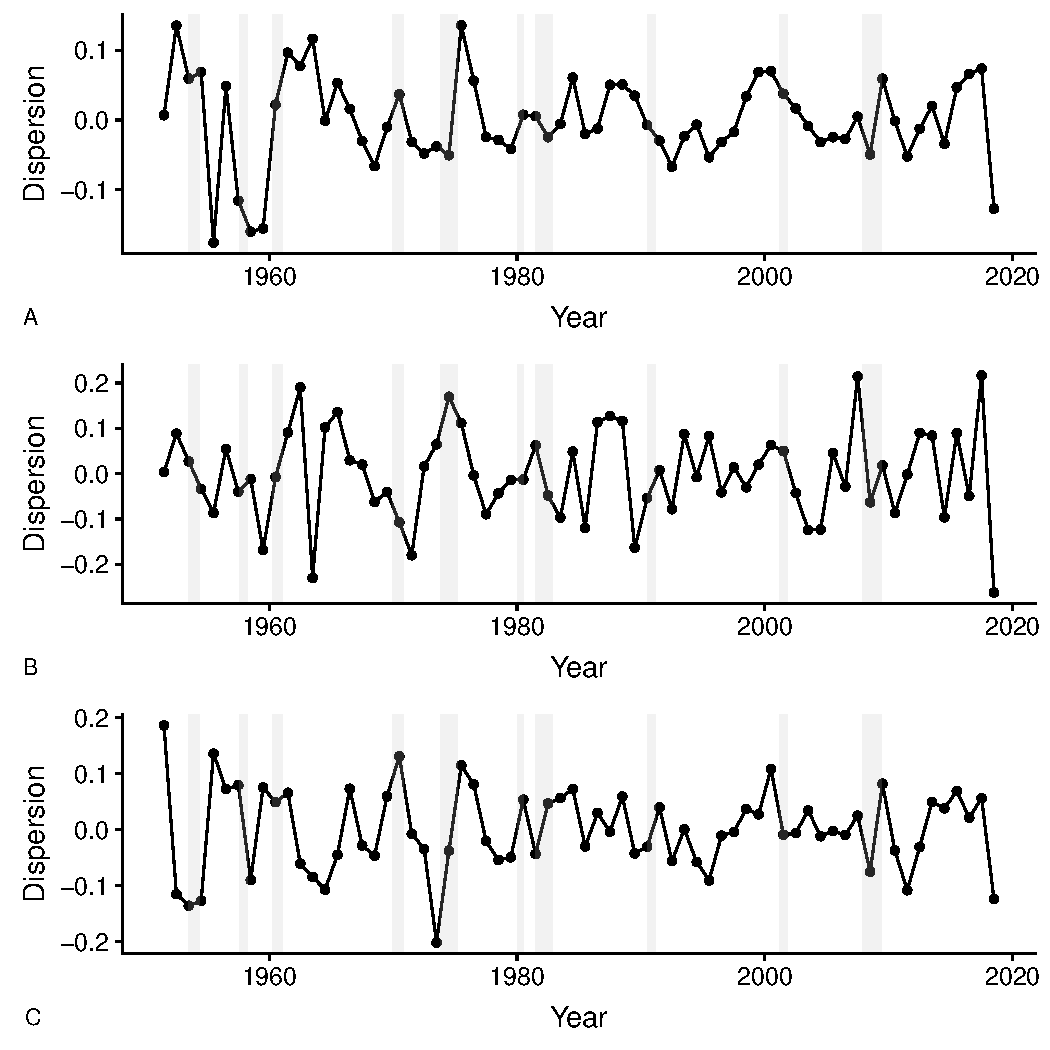
\includegraphics[width=0.8\textwidth]{figure/unnamed-chunk-1-1} 

}

\begin{table}[!htbp] \centering 
  \caption{Results} 
  \label{} 
\begin{tabular}{@{\extracolsep{5pt}}lD{.}{.}{-3} } 
\\[-1.8ex]\hline 
\hline \\[-1.8ex] 
 & \multicolumn{1}{c}{\textit{Dependent variable:}} \\ 
\cline{2-2} 
\\[-1.8ex] & \multicolumn{1}{c}{dayToDaySkills} \\ 
\hline \\[-1.8ex] 
 treatEF & 0.411^{***} \\ 
  & (0.081) \\ 
  & \\ 
 Constant & 2.598^{***} \\ 
  & (0.071) \\ 
  & \\ 
\hline \\[-1.8ex] 
Observations & \multicolumn{1}{c}{428} \\ 
R$^{2}$ & \multicolumn{1}{c}{0.057} \\ 
Adjusted R$^{2}$ & \multicolumn{1}{c}{0.055} \\ 
Residual Std. Error & \multicolumn{1}{c}{0.699 (df = 426)} \\ 
F Statistic & \multicolumn{1}{c}{25.932$^{***}$ (df = 1; 426)} \\ 
\hline 
\hline \\[-1.8ex] 
\textit{Note:}  & \multicolumn{1}{r}{$^{*}$p$<$0.1; $^{**}$p$<$0.05; $^{***}$p$<$0.01} \\ 
\end{tabular} 
\end{table}

\end{knitrout}
\floatfoot{Note: Time series plots of approximate deviations of the three annual dispersion measures from their trends in percent. A shows the full sample, B the non-durable manufacturing sector, and C the durable manufacturing sector. After taking the natural logarithm of the dispersion measures defined in equation 1, I have isolated their cyclical components with an HP-100 filter. The shaded bars represent recessions as defined by the NBER. The year ticks refer to January 1. The dispersion measures take as their date the middle of the year, July 2. Compare Kehrig (2015), Figure 1.}
\end{figure}



%\printbibliography
\end{document}
